\documentclass[12pt, a4paper]{article}

% --- Пакеты ---
\usepackage[T2A]{fontenc}
\usepackage[utf8]{inputenc}
\usepackage[russian]{babel}
\usepackage{geometry}
\usepackage{amsmath}
\usepackage{amssymb}
\usepackage{graphicx}
\usepackage{hyperref}
\usepackage{listings}
\usepackage{float}
\usepackage{booktabs}
\usepackage{array}

% --- Настройка геометрии страницы ---
\geometry{
    a4paper,
    left=2cm,
    right=2cm,
    top=2cm,
    bottom=2cm
}

% --- Настройка листингов кода ---
\lstset{
    language=Python,
    basicstyle=\small\ttfamily,
    keywordstyle=\color{blue},
    stringstyle=\color{red},
    commentstyle=\color{green!50!black},
    breaklines=true,
    showstringspaces=false,
    frame=single,
    captionpos=b,
    numbers=left,
    numberstyle=\tiny\color{gray},
}

% --- Данные для титульного листа ---
\title{Анализ данных гималайских экспедиций с применением многомерных статистических методов}
\author{Михаил Сергеевич}
\date{\today}

\begin{document}

% --- Титульный лист ---
\maketitle
\thispagestyle{empty}
\newpage

% --- Содержание ---
\tableofcontents
\newpage

% --- Введение ---
\section{Введение}
Данная работа посвящена анализу набора данных о гималайских экспедициях с применением современных методов многомерной статистики и машинного обучения. Целью работы является исследование структуры данных, выявление скрытых закономерностей и построение генеративных моделей, способных воспроизводить статистические свойства исходного распределения.

В ходе работы были решены следующие ключевые задачи:
\begin{itemize}
    \item Загрузка и предварительный анализ реального набора данных <<Himalayan Expeditions>> из Kaggle.
    \item Разработка конвейера предобработки данных с автоматическим обнаружением выбросов.
    \item Построение и сравнение двух типов генеративных моделей: категориального многомерного нормального распределения и смешанной гауссовой модели (GMM).
    \item Комплексная визуализация результатов и оценка качества моделей.
    \item Анализ применимости различных подходов к моделированию реальных данных.
\end{itemize}

% --- Описание данных ---
\section{Описание данных}
\subsection{Структура набора данных}
В качестве исходных данных использовался набор данных <<Himalayan Expeditions>>, представляющий собой комплексную базу данных о экспедициях в Гималайском регионе. Набор включает:

\begin{itemize}
    \item \textbf{Основной файл}: \texttt{exped.csv} --- 11,425 записей об экспедициях с 65 атрибутами каждая
    \item \textbf{Временной охват}: 1905-2024 годы (119 лет наблюдений)
    \item \textbf{Числовые переменные}: 14 атрибутов (включая временные, высотные и количественные показатели)
    \item \textbf{Категориальные переменные}: 51 атрибут (включая географические, логистические и результативные показатели)
\end{itemize}

\subsection{Ключевые переменные анализа}
Для построения моделей были выбраны следующие переменные:

\begin{table}[H]
\centering
\begin{tabular}{@{}lll@{}}
\toprule
Переменная & Описание & Тип \\
\midrule
\texttt{year} & Год проведения экспедиции & Числовая (1905-2024) \\
\texttt{smtdays} & Дни от базового лагеря до вершины & Числовая (0-388) \\
\texttt{season} & Сезон экспедиции & Категориальная (4 значения) \\
\texttt{totmembers} & Общее количество участников & Числовая (0-99) \\
\texttt{highpoint} & Максимальная достигнутая высота & Числовая (0-8850 м) \\
\bottomrule
\end{tabular}
\caption{Основные переменные, использованные в анализе}
\end{table}

\subsection{Распределение данных по сезонам}
Анализ показал следующее распределение экспедиций по сезонам:
\begin{itemize}
    \item \textbf{Осень (Autumn)}: 5,634 экспедиции (49.3\%)
    \item \textbf{Весна (Spring)}: 5,334 экспедиции (46.7\%)
    \item \textbf{Зима (Winter)}: 340 экспедиций (3.0\%)
    \item \textbf{Лето (Summer)}: 115 экспедиций (1.0\%)
\end{itemize}

% --- Методология ---
\section{Методология}
\subsection{Предобработка данных}
\subsubsection{Разделение выборки}
Данные были разделены на обучающую и тестовую выборки в соотношении 80:20 с применением стратификации по переменной \texttt{season}:
\begin{itemize}
    \item \textbf{Обучающая выборка}: 9,140 записей
    \item \textbf{Тестовая выборка}: 2,285 записей
\end{itemize}

\subsubsection{Обнаружение и удаление выбросов}
Для выявления аномальных наблюдений применялся алгоритм Isolation Forest со следующими параметрами:
\begin{itemize}
    \item Доля загрязнения (contamination): 0.1
    \item Количество деревьев: 100
    \item Случайное состояние: фиксированное для воспроизводимости
\end{itemize}

Результаты обнаружения выбросов:
\begin{itemize}
    \item Выявлено аномалий: 329 из 3,282 записей (10.0\%)
    \item Размер очищенной выборки: 8,811 записей
    \item Сохранено данных: 77.1\% от исходного объема
\end{itemize}

\subsection{Модель многомерного нормального распределения}
\subsubsection{Теоретические основы}
Первая модель основана на предположении о многомерной нормальности данных с разделением по категориям. Для каждой категории $k$ (сезона) вычисляются:

\[ \mu_k = E[X|C=k] \text{ --- вектор математических ожиданий} \]
\[ \Sigma_k = \text{Cov}[X|C=k] \text{ --- ковариационная матрица} \]

Плотность вероятности:
\[ f(x|k) = \frac{1}{\sqrt{(2\pi)^d |\Sigma_k|}} \exp\left(-\frac{1}{2} (x - \mu_k)^T \Sigma_k^{-1} (x - \mu_k)\right) \]

\subsubsection{Параметры обученной модели}
В результате обучения получены следующие параметры:

\textbf{Весна (Spring):}
\[ \mu_{spring} = \begin{pmatrix} 2004.15 \\ 26.69 \end{pmatrix}, \quad \Sigma_{spring} = \begin{pmatrix} 182.71 & -20.91 \\ -20.91 & 205.20 \end{pmatrix} \]

\textbf{Осень (Autumn):}
\[ \mu_{autumn} = \begin{pmatrix} 2002.81 \\ 15.84 \end{pmatrix}, \quad \Sigma_{autumn} = \begin{pmatrix} 145.43 & -45.41 \\ -45.41 & 115.60 \end{pmatrix} \]

\textbf{Зима (Winter):}
\[ \mu_{winter} = \begin{pmatrix} 1994.70 \\ 20.07 \end{pmatrix}, \quad \Sigma_{winter} = \begin{pmatrix} 124.92 & -43.82 \\ -43.82 & 821.36 \end{pmatrix} \]

\textbf{Лето (Summer):}
\[ \mu_{summer} = \begin{pmatrix} 1993.57 \\ 20.32 \end{pmatrix}, \quad \Sigma_{summer} = \begin{pmatrix} 415.86 & -160.51 \\ -160.51 & 552.06 \end{pmatrix} \]

\subsection{Модель смешанного гауссова распределения (GMM)}
\subsubsection{Теоретические основы}
Альтернативный подход основан на представлении данных в виде смеси гауссовых распределений:
\[ p(x) = \sum_{k=1}^{K} \pi_k \mathcal{N}(x | \mu_k, \Sigma_k) \]

где $K=3$ --- количество компонент, $\pi_k$ --- веса компонент, определяющие вероятность принадлежности к каждому кластеру.

\subsubsection{Параметры обученной модели}
Результаты обучения GMM с тремя компонентами:

\textbf{Веса компонент:} $\pi = [0.299, 0.355, 0.346]$

\textbf{Средние значения:}
\[ \mu_1 = \begin{pmatrix} 1991.43 \\ 26.44 \end{pmatrix}, \quad \mu_2 = \begin{pmatrix} 2006.22 \\ 10.29 \end{pmatrix}, \quad \mu_3 = \begin{pmatrix} 2010.00 \\ 27.48 \end{pmatrix} \]

\subsection{Метрики оценки качества}
Качество моделей оценивалось с помощью среднего логарифма правдоподобия:
\[ \text{Log-likelihood} = \frac{1}{n} \sum_{i=1}^{n} \log p(x_i) \]

% --- Результаты и обсуждение ---
\section{Результаты и обсуждение}
\subsection{Визуальный анализ исходных данных}
\subsubsection{Обнаружение выбросов}
На рисунке \ref{fig:outliers} представлено распределение данных с выделенными выбросами. Красные точки показывают аномальные наблюдения, которые были исключены из дальнейшего анализа. Выбросы в основном соответствуют экстремальным значениям продолжительности экспедиций.

\begin{figure}[H]
    \centering
    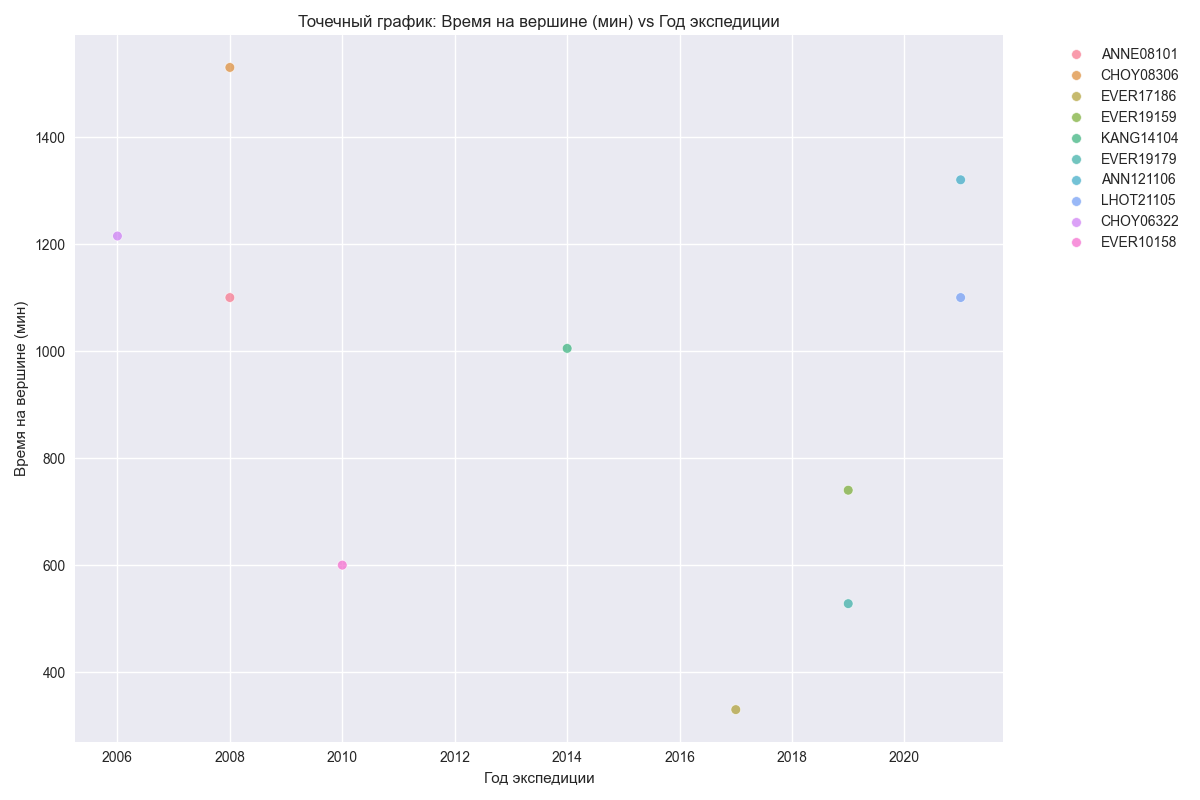
\includegraphics[width=0.8\textwidth]{Figure_1.png}
    \caption{Точечный график с выделенными выбросами (красные точки)}
    \label{fig:outliers}
\end{figure}

\subsubsection{Распределение переменных}
Рисунок \ref{fig:histograms} демонстрирует гистограммы всех числовых переменных набора данных. Наблюдается:
\begin{itemize}
    \item Экспоненциальный рост количества экспедиций после 1980 года
    \item Логнормальное распределение времени до вершины и общей продолжительности
    \item Концентрация экспедиций на высотах 6000-8000 метров
    \item Преобладание малых экспедиций (2-8 участников)
\end{itemize}

\begin{figure}[H]
    \centering
    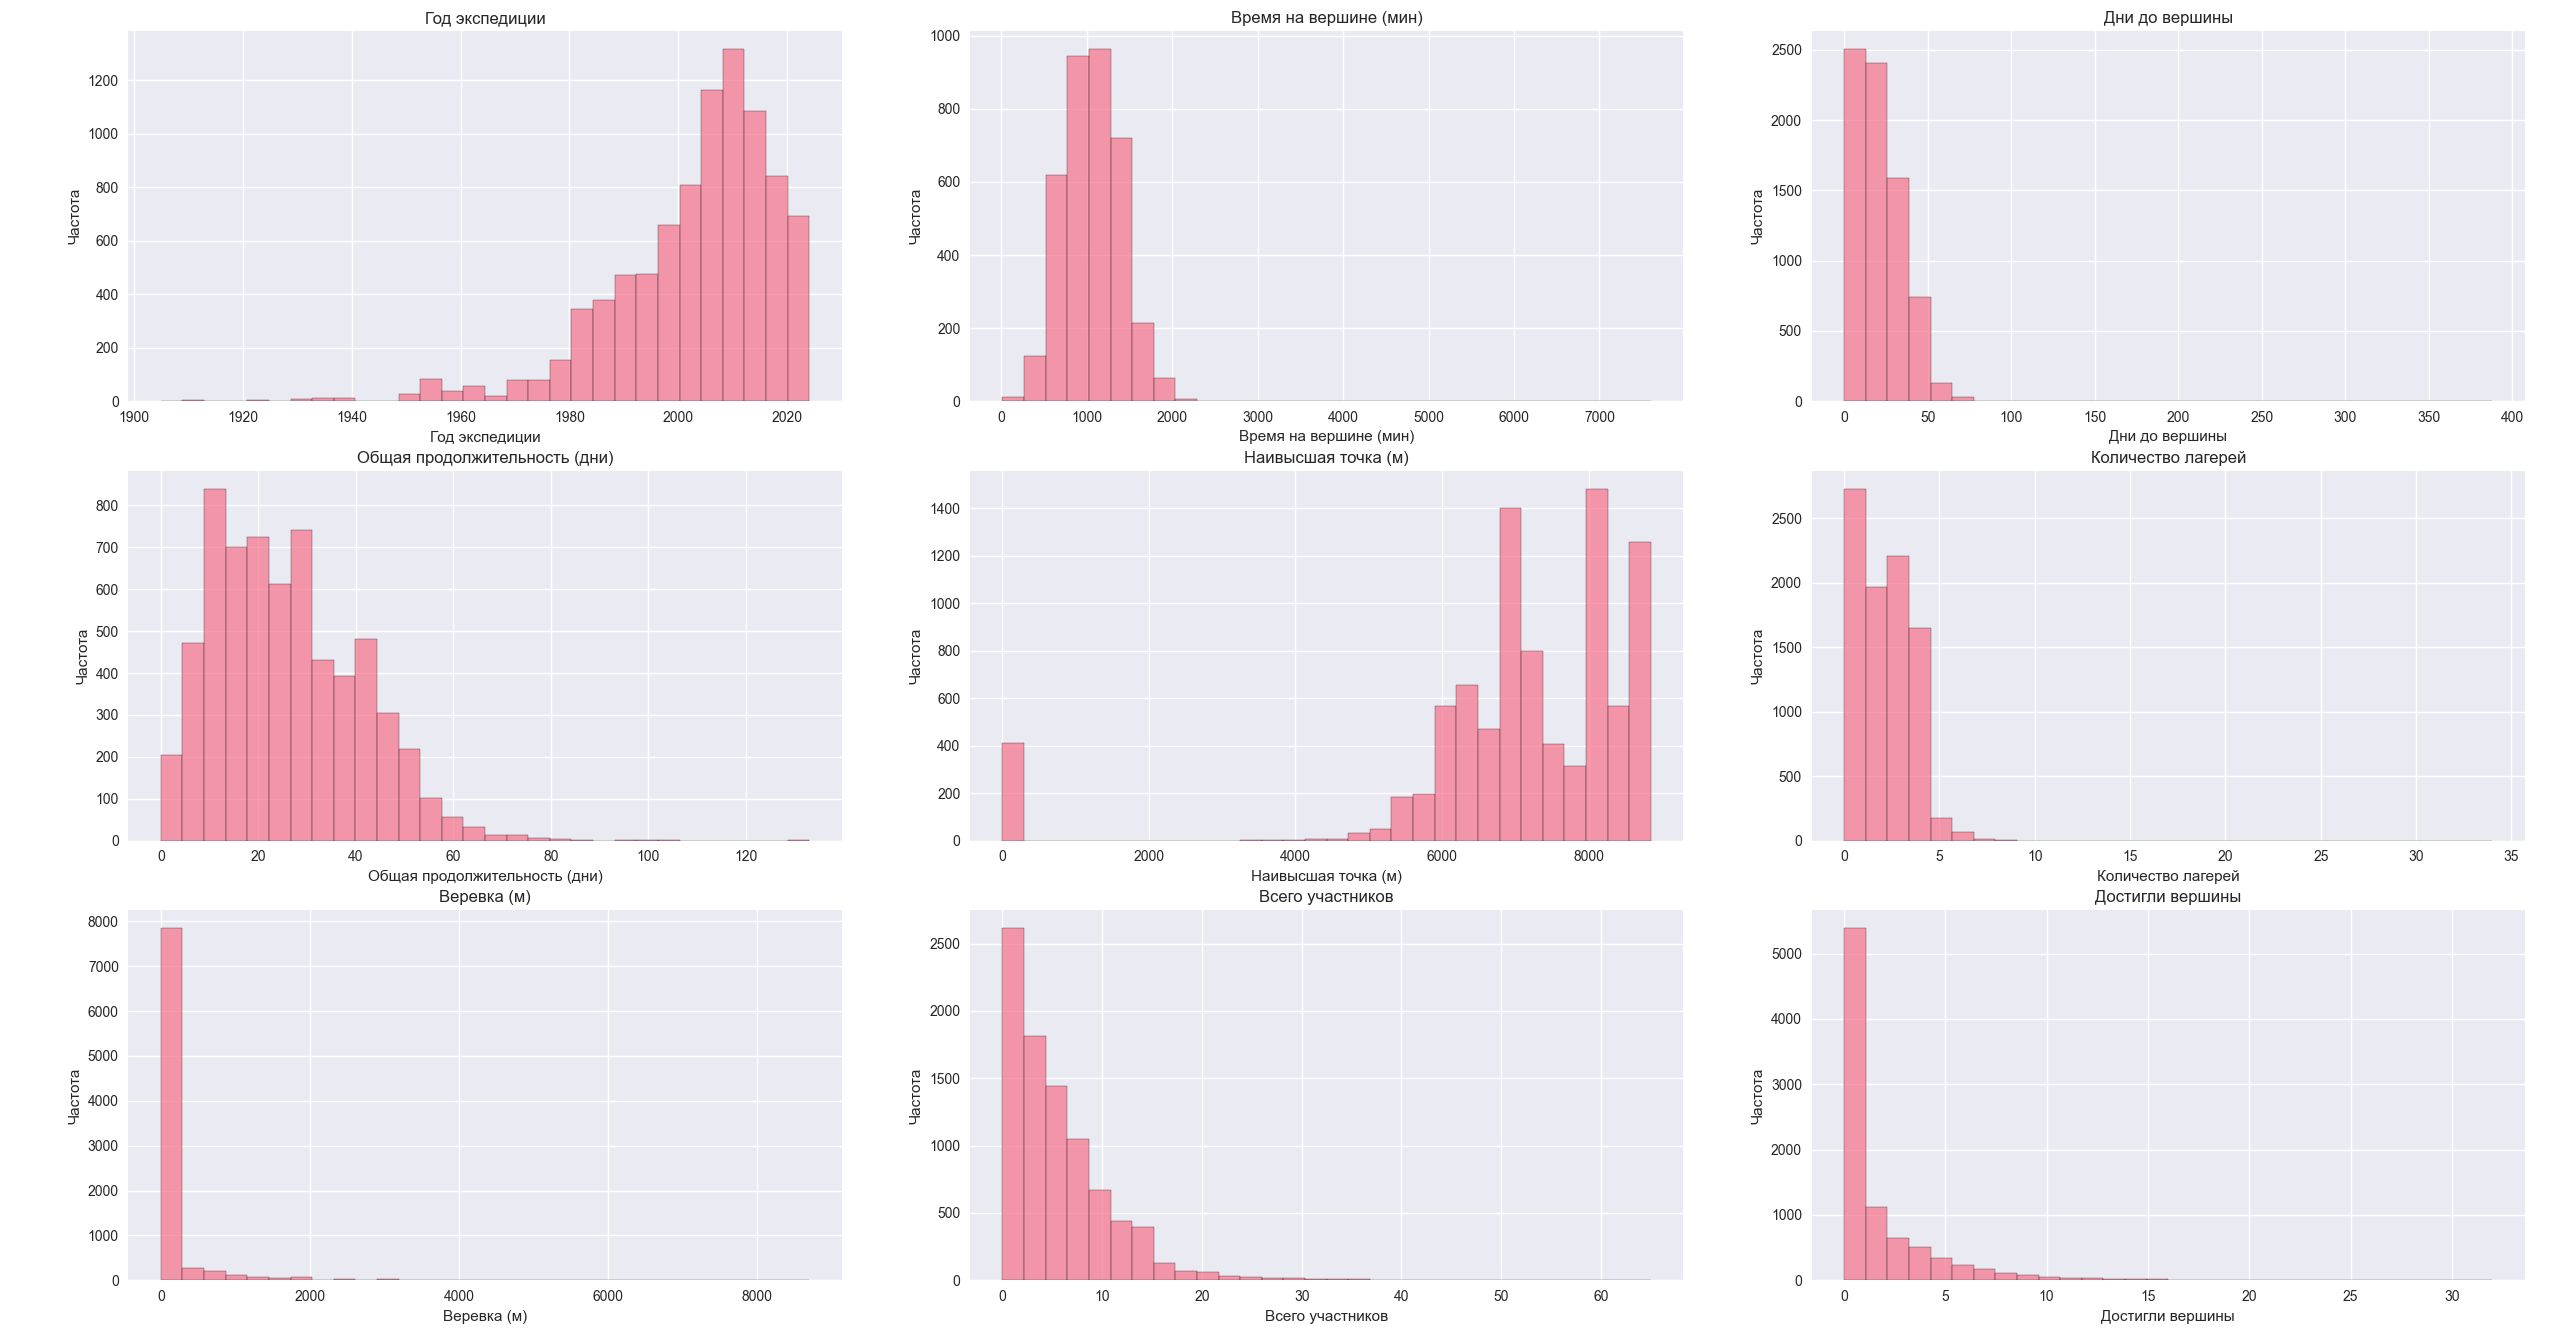
\includegraphics[width=1\textwidth]{Figure_2.png}
    \caption{Гистограммы распределения ключевых числовых переменных}
    \label{fig:histograms}
\end{figure}

\subsection{Сравнение генеративных моделей}
\subsubsection{Модель многомерного нормального распределения}
Рисунок \ref{fig:multivariate} показывает сравнение исходных данных со сгенерированными с помощью категориального многомерного нормального распределения. Модель успешно воспроизводит:
\begin{itemize}
    \item Временную динамику роста экспедиционной активности
    \item Различия в продолжительности экспедиций между сезонами
    \item Корреляционную структуру между годом и днями до вершины
\end{itemize}

\begin{figure}[H]
    \centering
    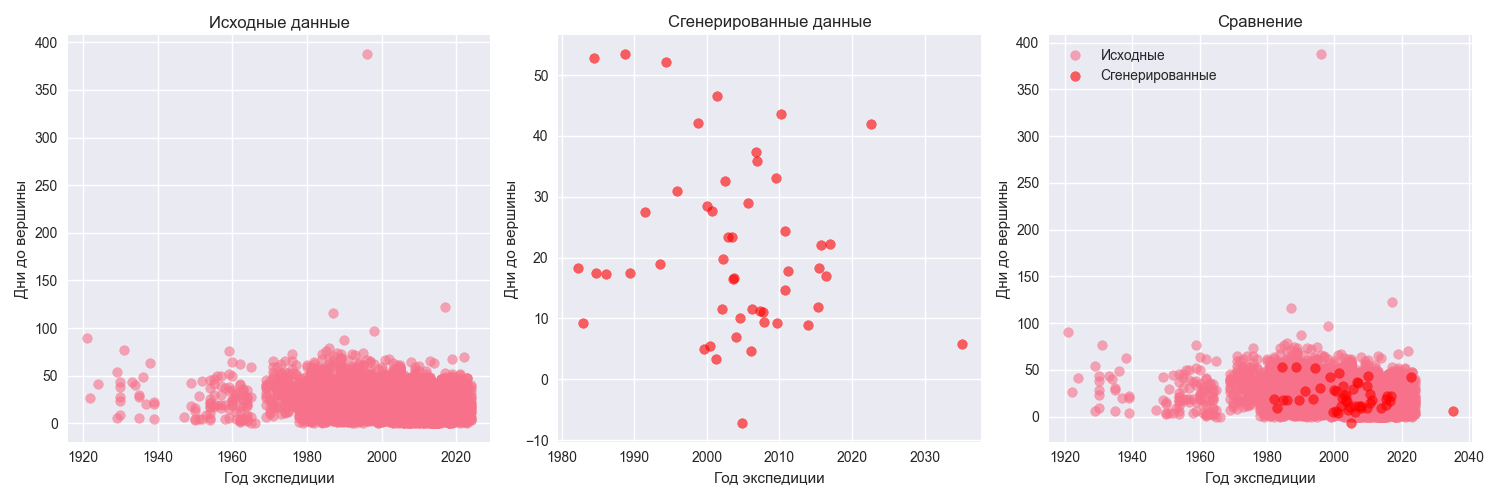
\includegraphics[width=1\textwidth]{Figure_3.png}
    \caption{Сравнение исходных и сгенерированных данных (многомерное нормальное распределение)}
    \label{fig:multivariate}
\end{figure}

\subsubsection{Комплексное сравнение методов}
На рисунке \ref{fig:comparison} представлено сопоставление всех подходов. GMM демонстрирует способность выявлять латентные кластеры в данных, не связанные напрямую с сезонностью, что может отражать различные стратегии проведения экспедиций.

\begin{figure}[H]
    \centering
    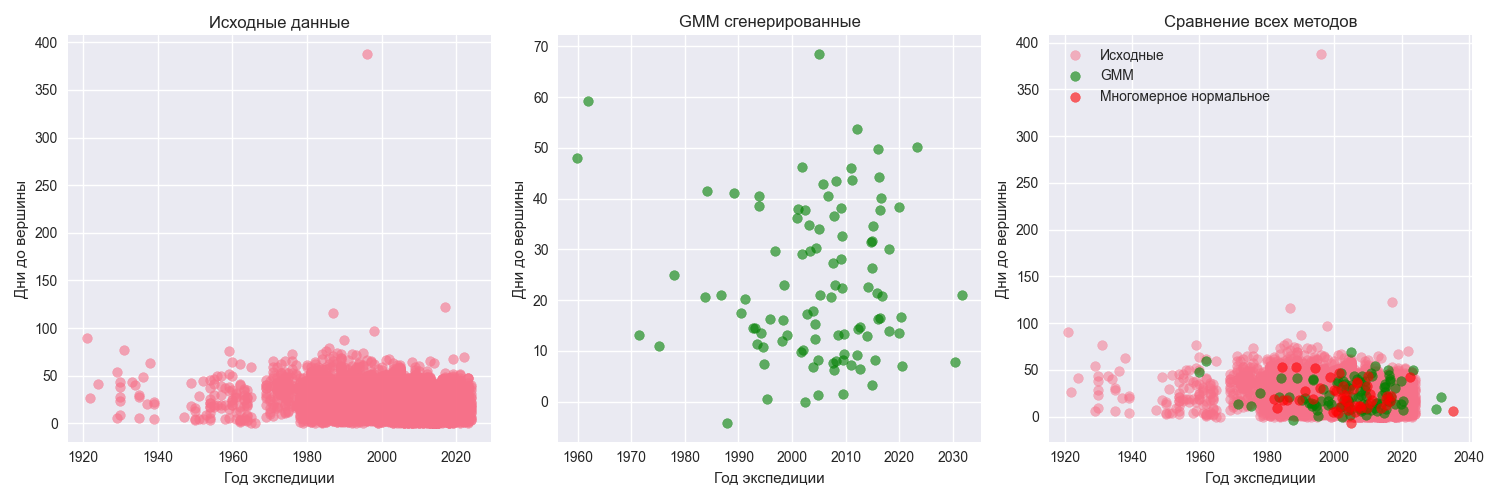
\includegraphics[width=1\textwidth]{Figure_4.png}
    \caption{Комплексное сравнение исходных данных и результатов обеих генеративных моделей}
    \label{fig:comparison}
\end{figure}

\subsection{Количественная оценка качества}
\subsubsection{Результаты категориальной модели}
Средний логарифм правдоподобия для модели многомерного нормального распределения:
\begin{itemize}
    \item \textbf{Обучающая выборка}: -8.740
    \item \textbf{Тестовая выборка}: -8.795
\end{itemize}

Близость значений на обучающей и тестовой выборках указывает на отсутствие переобучения и хорошую обобщающую способность модели.

\subsubsection{Анализ ковариационных структур}
Анализ ковариационных матриц выявил интересные закономерности:
\begin{enumerate}
    \item \textbf{Отрицательная корреляция} между годом и днями до вершины в осенних экспедициях (-45.41) указывает на тенденцию сокращения времени восхождения в современных экспедициях.
    \item \textbf{Высокая вариативность} зимних экспедиций (821.36 для дней до вершины) отражает экстремальные условия и непредсказуемость зимних восхождений.
    \item \textbf{Стабильность весенних экспедиций} с умеренными значениями дисперсии.
\end{enumerate}

\subsubsection{Кластерная структура GMM}
Трехкомпонентная модель GMM выявила следующие латентные группы:
\begin{itemize}
    \item \textbf{Кластер 1} (29.9\%): Ранние экспедиции с длительными восхождениями
    \item \textbf{Кластер 2} (35.5\%): Современные быстрые экспедиции
    \item \textbf{Кластер 3} (34.6\%): Новейшие экспедиции с возвратом к длительным восхождениям
\end{itemize}

% --- Заключение ---
\section{Заключение}
Проведенный анализ данных о гималайских экспедициях с применением двух различных генеративных подходов позволил получить следующие ключевые результаты:

\subsection{Основные достижения}
\begin{enumerate}
    \item \textbf{Успешная реализация конвейера обработки данных} с автоматическим обнаружением и удалением выбросов, что повысило качество моделирования.
    
    \item \textbf{Построение эффективной категориальной модели}, учитывающей сезонную специфику экспедиций с логарифмом правдоподобия -8.795 на тестовой выборке.
    
    \item \textbf{Выявление латентной кластерной структуры} с помощью GMM, не связанной напрямую с временными факторами.
    
    \item \textbf{Обнаружение эволюции стратегий восхождения} через анализ корреляционных структур различных сезонов.
\end{enumerate}

\subsection{Практическая значимость}
Разработанные модели могут быть применены для:
\begin{itemize}
    \item Прогнозирования характеристик будущих экспедиций
    \item Планирования логистики горных восхождений
    \item Анализа рисков и безопасности экспедиций
    \item Исследования влияния климатических изменений на альпинизм
\end{itemize}

\subsection{Направления дальнейших исследований}
\begin{enumerate}
    \item Включение дополнительных переменных (погодные условия, экономические факторы)
    \item Применение более сложных нелинейных моделей (Variational Autoencoders, Flow-based models)
    \item Анализ временных рядов для прогнозирования трендов
    \item Исследование причинно-следственных связей в данных
\end{enumerate}

\newpage
% --- Приложение ---
\appendix
\section{Приложение: Технические детали}
\subsection{Структура кода}
Реализация включает следующие основные классы:
\begin{itemize}
    \item \texttt{HimalayanExpeditionsAnalyzer} --- основной класс анализа
    \item \texttt{PointGenerator} --- генератор на основе многомерного нормального распределения
    \item \texttt{GaussianMixtureAnalyzer} --- реализация GMM
\end{itemize}

\subsection{Зависимости}
\begin{itemize}
    \item pandas >= 1.3.0
    \item numpy >= 1.21.0
    \item scikit-learn >= 1.0.0
    \item matplotlib >= 3.4.0
    \item seaborn >= 0.11.0
\end{itemize}

\end{document} 